\documentclass[11pt]{beamer}
\usepackage[utf8]{inputenc}
\usepackage[german]{babel}
\usepackage{amsmath}
\usetheme{default}
\setbeamertemplate{footline}[frame number]
\begin{document}
	\author{Gerald ..., Moritz ..., Tim Herbermann, Sebastian Siebert}
	\title{Akustik}
	\subtitle{eine Versuchsreihe}
	%\logo{}
	%\institute{}
	%\date{}
	%\subject{}
	%\setbeamercovered{transparent}
	%\setbeamertemplate{navigation symbols}{}
	\frame[plain]{\maketitle}
	
	\begin{frame}
		\frametitle{Einleitung}
		Seite 1
	\end{frame}
	\begin{frame}
		\frametitle{Schall}
		Seite 2
	\end{frame}
	\begin{frame}
		\frametitle{Laufzeitmessung \qquad Veruschsaufbau}
		\begin{figure}
			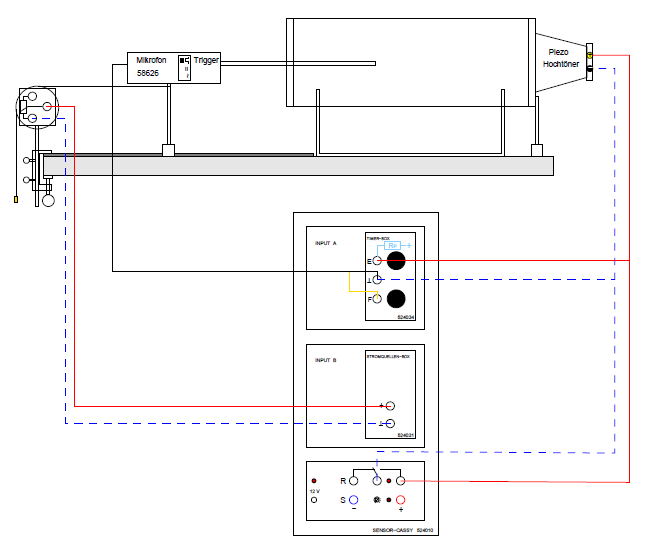
\includegraphics[width=\linewidth]{aufbau_laufzeitmessung}
		\end{figure}
	\end{frame}
\end{document}